\documentclass{article}

\usepackage[final]{neurips_2019}
\usepackage[utf8]{inputenc} % allow utf-8 input
\usepackage[T1]{fontenc}    % use 8-bit T1 fonts
\usepackage{hyperref}       % hyperlinks
\usepackage{url}            % simple URL typesetting
\usepackage{booktabs}       % professional-quality tables
\usepackage{amsfonts}       % blackboard math symbols
\usepackage{nicefrac}       % compact symbols for 1/2, etc.
\usepackage{microtype}      % microtypography
\usepackage{graphicx}
\usepackage{subfig}
\usepackage{natbib}
\usepackage{float}
\usepackage{algpseudocode,algorithm}

\usepackage{multicol}
\setlength{\columnsep}{1cm}

\usepackage{hyperref}
\hypersetup{
    colorlinks=true,
    linkcolor=blue,
    filecolor=magenta,      
    urlcolor=cyan,
}

\usepackage{caption}
\captionsetup[table]{labelsep=space}
\captionsetup[figure]{labelsep=space}
\newcommand{\mycaption}[2]{\caption[#1]{\textbf{#1.} #2}}

\title{Residual Attention Network for Image Classification}

\author{%
  Shengjie Sun \\
  ss5593\\
  Department of Statistics\\
  Columbia University\\
  New York, NY 10027 \\
  \texttt{ss5593@columbia.edu} \\
  % examples of more authors
  \And
  Yiming Tan \\
  xx9999 \\
  Department of Statistics\\
  Columbia University\\
  New York, NY 10027 \\
  \texttt{xx9999@columbia.edu} \\
  \And
  Feng Su \\
  xx9999 \\
  Department of Statistics\\
  Columbia University\\
  New York, NY 10027 \\
  \texttt{xx9999@columbia.edu}
}

\begin{document}

\maketitle

\begin{multicols}{2}
\section*{Abstract}
\textit{In this project, we reimplement a convolutional neural network structure called "Residual Attention Network" proposed by \citet{wang2017residual}. The great power of attention in machine translation has indicated by \citet{vaswani2017attention} and thus we are curious how the attention can influence the image classification task. During investigating the idea of residual attention, the main challenging is that the network is too flexible to choose a good hyper-parameters and the time and computing resources is limited for a network with such many residual blocks.}




\section{Introduction}
As the authors, \citet{vaswani2017attention}, of the paper mentioned, the residual mechanism in the image classification can serve to both focused location selection and the enhancement of the representations of focused objects. After the network structure like VGG given by \cite{simonyan2014very} and the improvement of computing resources, the newer networks are mostly deeper, as the structure proposed by this paper. Basically, residual attention network is a very deep convolutional neural network connected by residual unit mixed with soft mask, so called attention in this paper. 

As for our project, first we want to implement the idea of this paper in tensorflow 2 and then compared our result and the result in the paper. Furthermore, we try to exam what should be a good "attention" for the image classification, the attention mentioned in this paper is actually a soft mask for a feature, which is quite different from the word "attention" used in the area of natural language processing. 
\end{multicols}

\begin{figure}[!htb]  
\centering  
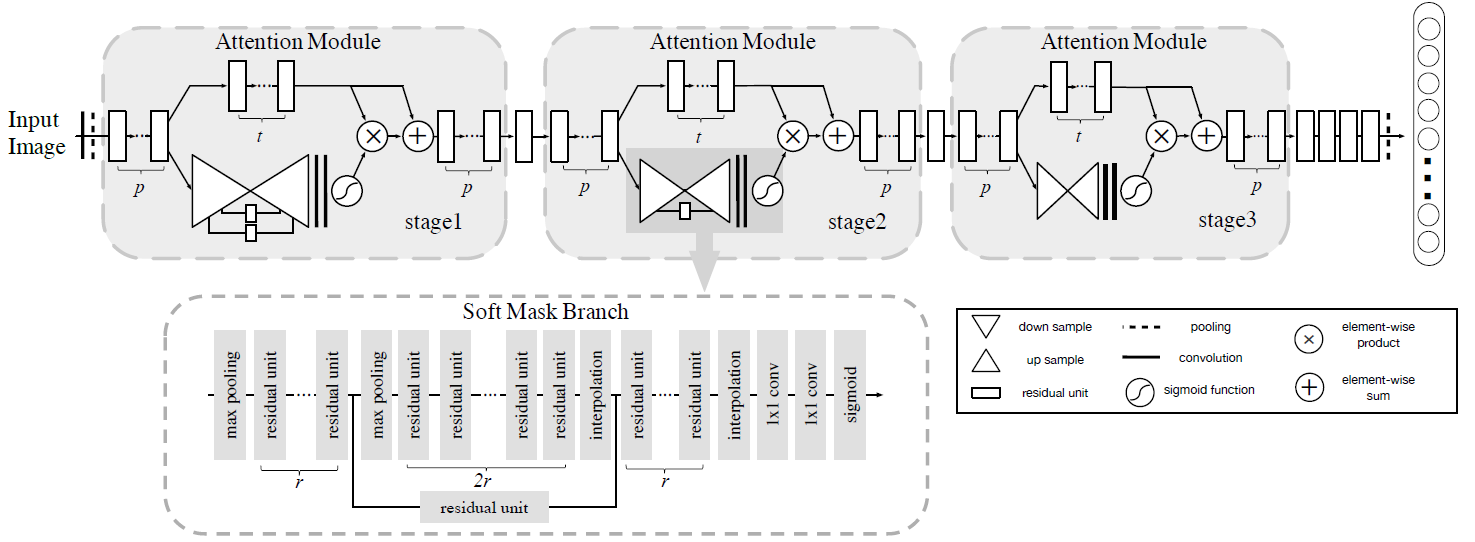
\includegraphics[width=6in]{imgs/attention_module_stage2.png}  
\mycaption{Example architecture of the residual attention network.}{We use three hyper-parameters for the design of Attention Module: p, t and r. The hyper-parameter p denotes the number of pre-processing Residual Units before splitting into trunk branch and mask branch. t denotes the number of Residual Units in trunk branch. r denotes the number of Residual Units between adjacent pooling layer in the mask branch. In our experiments, we use the following hyper-parameters setting: {p = 1, t = 2, r = 1}. The number of channels in the soft mask Residual Unit and corresponding trunk branches is the same.}  
\label{fig:attention_module_stage2}
\end{figure}

\newpage
\begin{multicols}{2}
There are several challenges and difficulties for this project. First of all, there are so many implementation details are not provided by the original paper. For example, there are so many residual units in one attention module but what is exactly the structure and parameters setting of the residual unit? Are all the residual units same? The second main challenging is that the model is relative huge considering the computer resources we have. Even thought it is feasible to train a model throughout several times, but the structure of attention module is such flexible, it is not very easy to find a good selection of hyper-parameters. 

Our solution to the first difficulty is to give a model with similar size of parameters. Even thought there are many details, the skeleton of the structure is clear. Therefore, we tried to give an implementation with similar size of parameters. The solution to the second one is that we tried as many acceleration methods as we can to squeeze our computation ability. And we also sacrificed some accuracy based on the real situation. 
\section{Summary of the Original Paper}
\subsection{Methodology of the Original Paper}
The key idea of the whole paper lies on the structure of attention module and it can be roughly summarized by the following formula:
\begin{eqnarray*}
H_{i,c}(x)&=&(1+M_{i,c}(x))*T_{i, c}(x) \\
&=&T_{i, c}(x) + M_{i,c}(x)*T_{i, c}(x)
\label{eqn:attention_module}
\end{eqnarray*}
$T(x)$ is the common feed forward layers while $M(x)$ ranges from [0, 1] and serves as feature selectors. 

If we consider $M_{i,c}(x)*T_{i, c}(x)$ as $x$, it would be exactly the same as residual learning. But it is indeed based on attention structure, and thus called residual attention network.

\begin{figure}[H] 
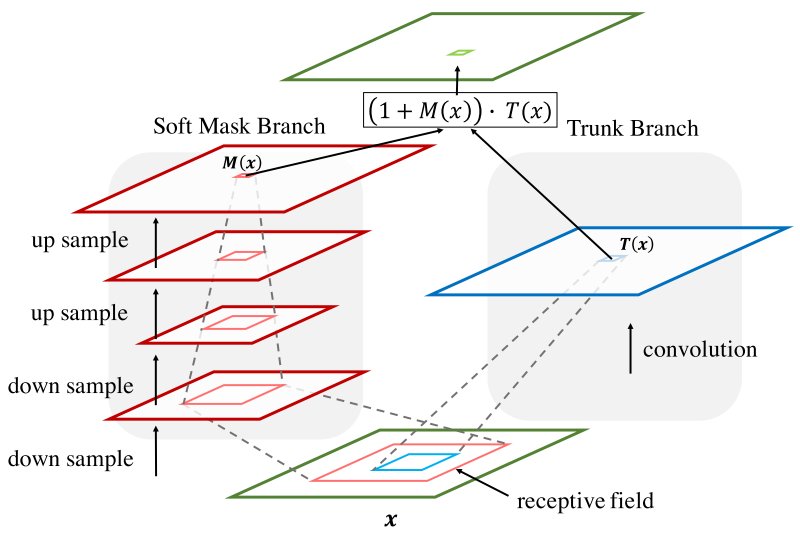
\includegraphics[width=3in]{imgs/receptive_field.png}  
\mycaption{Structure of Attention Module.}{$T(x)$ indicates the features generated by deep convolutional networks. $M(x)$ is the mask branche which work as feature selectors that enhance good features and suppress noises from trunk features.}  
\label{fig:receptive_field}
\end{figure}

\subsection{Key Results of the Original Paper}
\subsubsection{Residual structure benefits}
This paper argues that utilizing residual structure enables the stacking of more attention modules as shown in Figure \ref{fig:cifar10_residual}. This is not surprising us too much as this is just why residual learning, i.e. skipping connection, is so popular and useful.
\begin{figure}[H] 
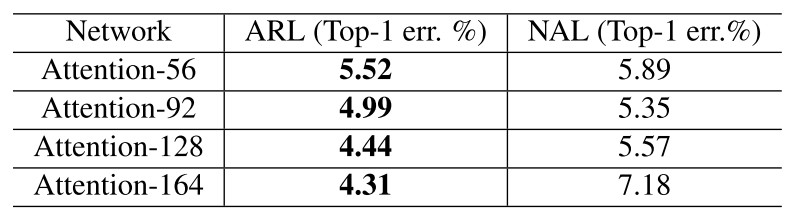
\includegraphics[width=3in]{imgs/cifar10_residual.png}  
\mycaption{Classification error (\%) on CIAFR-10.}{The networks trained using attention residual learning technique consistently outperform the networks trained with baseline method. The performance increases with the number of attention module when applying attention residual learning. In contrast, the performance of networks trained with “naive attention learning” method suffers obvious degradation.}  
\label{fig:cifar10_residual}
\end{figure}
The Figure \ref{fig:cifar10_stages} proved above argument in details, we can see that residual attention model has similar relative mean response to ResNet-164.
\begin{figure}[H] 
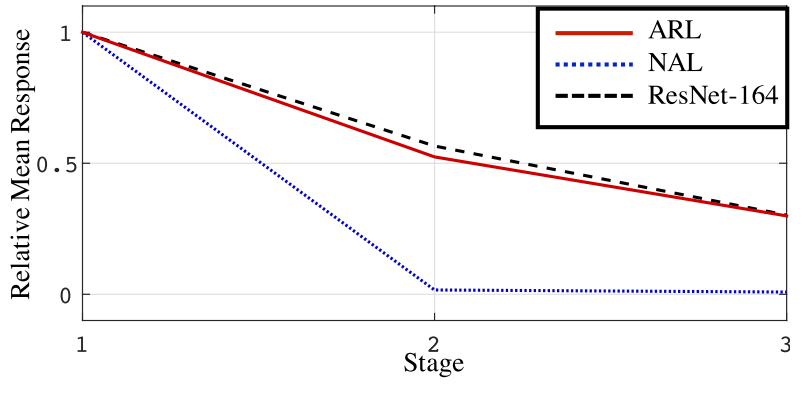
\includegraphics[width=3in]{imgs/cifar10_stages.png}  
\mycaption{The mean absolute response of output features in each stage.}{The response generated by the network trained using naive attention learning quickly vanishes in the stage 2 after four attention modules compared with network trained using attention residual learning.}  
\label{fig:cifar10_stages}
\end{figure}

\subsubsection{Attention structure benefits}
The paper shows that their model outperforms the state of art models. On the dataset CIFAR10 and CIFAR100, the attention residual learning scheme can effectively reduce the number of parameters in the network while enhancing the accuracy of the classification.

\begin{figure}[H] 
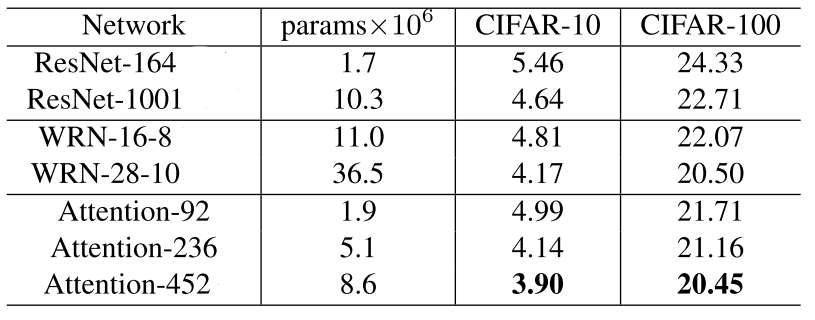
\includegraphics[width=3in]{imgs/cifar10_modes}  
\mycaption{Comparisons with state-of-the-art methods on CIFAR-10/100.}{}
\label{fig:cifar10_modes}
\end{figure}

\section{Methodology}
Basically, the model is constructed by attention modules shown in Figure \ref{fig:attention_module_stage2}. One attention module has two branches: trunk branch and soft mask branch. At each stage, there could be several attention modules and in Figure \ref{fig:attention_module_stage2}, each stage contains exactly one module. More specifically, in the soft mask branch, there are different number of skip connections between down sampling and up sampling layers. 

The paper did not provide the details of the residual unit and up or down sampling layers. But for the reimplementation, these details are crucial because we can not get the ImageNet dataset but for CIFAR10 or even CIFAR100, it is very easy to overfit. 

In our project, we tried to build so called Attention56 for CIFAR10, i.e. in each stage, there is only one attention module. The soft mask branch has two skip connections at stage 1, one skip connection at stage 2 and one at the last stage which is exactly same to to the Figure \ref{fig:attention_module_stage2}. We constructed two kind of residual unit. One required exactly the same identity mapping for the skip connection while the other allows the down sampling.  
 
\subsection{Objectives and Technical Challenges}
The main object is to get the accuracy as close as the one provided in the paper. But as mentioned several times, the details is important but hidden in this paper, so lots of experiments required but the time and computing resources limited. 

The other challenge is the coding writing, it is not difficult to build the overall structure for a specific model, say Attention56. But it is super time consuming to adjust the hyper-parameters. It is quite clear there are lots of sampling steps and skip connections. Therefore the dimension and the shape of images/tensors become a little bit annoying to keep consistent. Besides, the different model requires different attention model, at the end, the dimensions become chaos and requires lot of time to adjust. So, if you want to give codes which can reused for many models, it is somehow difficult to design. If not, there will be plenty of repeating codes that fixed the inputs and outputs dimension for each layers. 

The last but not least is how to prevent over-fitting. The learning ability of these model are high and over-fitting is common. Even there are so many skip connections, the over-fitting is still obvious. Finding a good way to prevent it for this kind of model structure is difficult for us. 

\subsection{Problem Formulation and Design}

\section{Implementation}
\subsection{Deep Learning Network}
\subsection{Software Design}

\section{Results}
\subsection{Project Results}
\subsection{Comparison of Results}
\subsection{Discussion of Insights Gained}

\section{Conclusion}
\section{Acknowledgement}

\end{multicols}

\newpage

\bibliography{citations}
\bibliographystyle{plainnat}
\end{document}